\subsection{Class Activation Maps}
We used pretrained network ResNet18 \cite{ResNet} from the \href{https://pytorch.org/}{torch} library. 
Since it already has a Global Average Pooling Layer after convolutional Layer, we directly create a hook at the forward pass. The heatmap superposed with image is created using \href{https://opencv.org/}{opencv}.
Other Networks which already have a GAP layer are Inception \cite{Inception}, SqueezeNet\cite{SqueezeNet}, and DensNet \cite{DensNet}.\\
For the labels, we used \cite{ILSVRC} dataset, a subset of ImageNet dataset available on Kaggle.
\begin{figure}[H]
    \centering
    \subfigure[]{
    \label{fig:Ex1}
    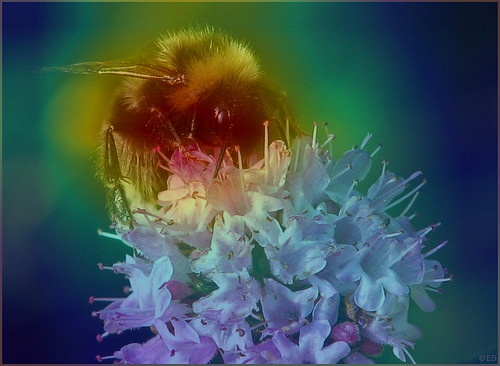
\includegraphics[width=.4\columnwidth]{CAM7.jpg}}
    \qquad
    \subfigure[]{
    \label{fig:Ex2}
    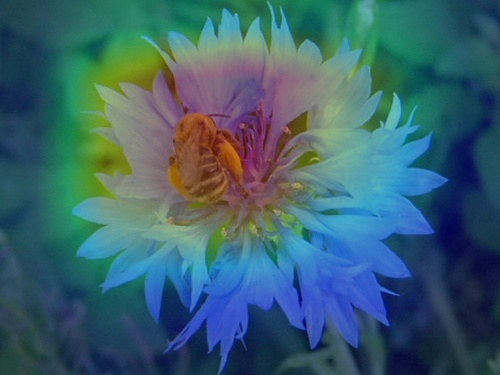
\includegraphics[width=.4\columnwidth]{CAM6.jpg}}
    \caption[Short text]{Some Examples with images of Bees}
    \label{fig:Some_Examples}
\end{figure}
This method showed remarkable results even when the softmax output scores of competing classes were really skewed.

\begin{figure}[H]
    \centering
    \subfigure[Golden Retriever \phantom{fdsfdsf} \phantom{fdsfdsf} Score=0.715]{
    \label{fig:Ex1}
    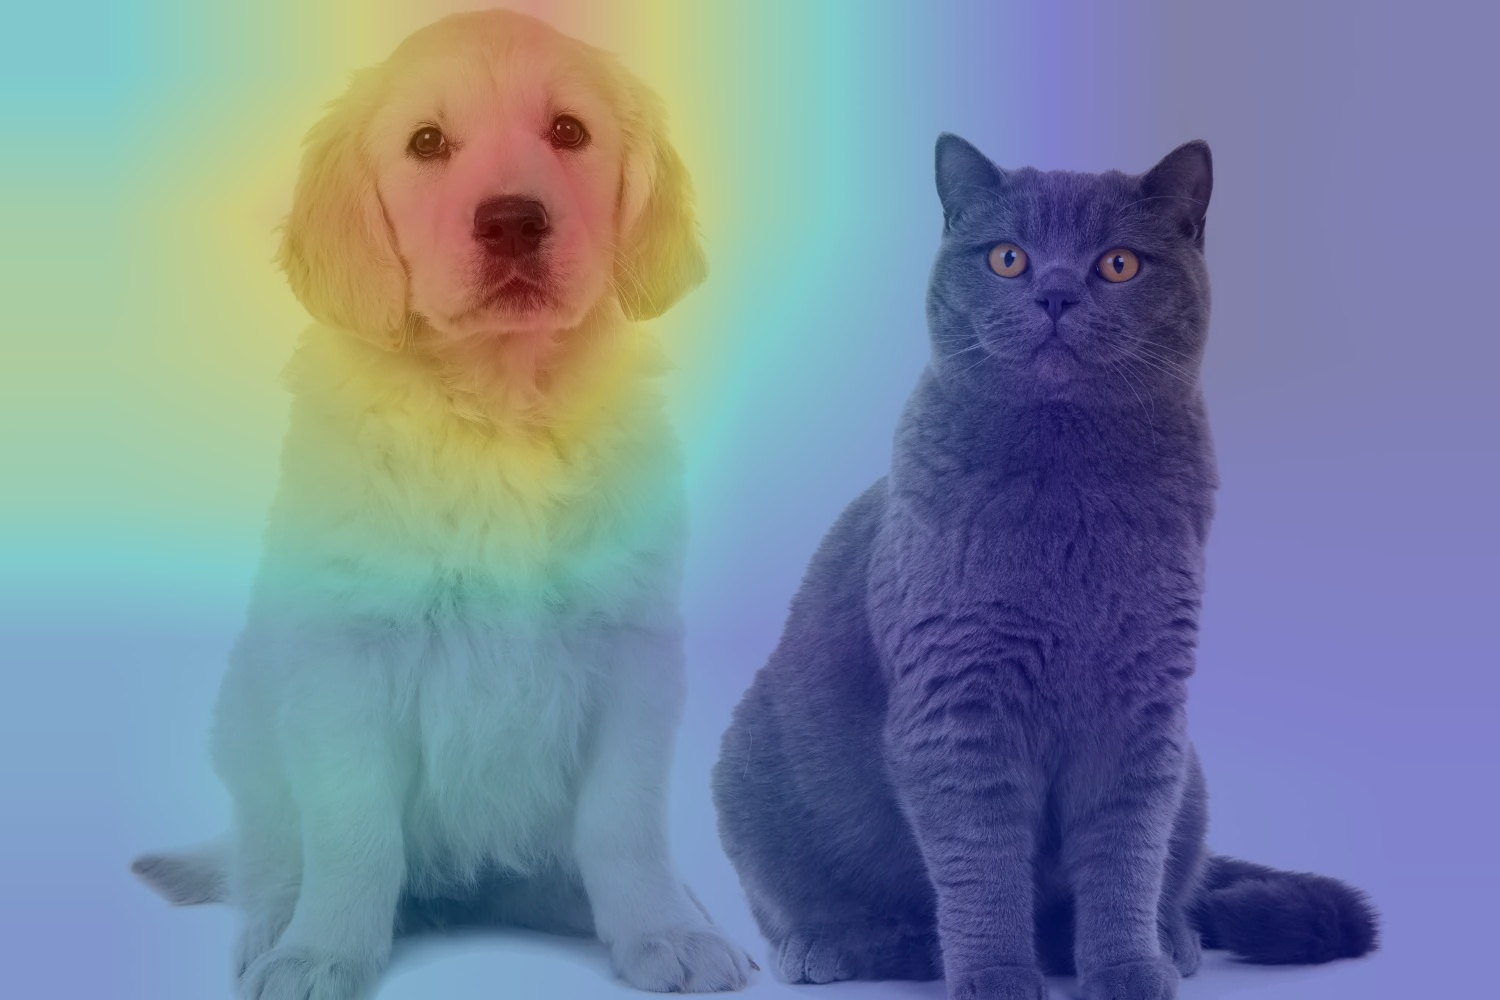
\includegraphics[width=.4\columnwidth]{CAM1.jpg}}
    \qquad
    \subfigure[Egyptian Mau \phantom{fdsfdsf} \phantom{fdsfdsf} Score=0.0021]{
    \label{fig:Ex1}
    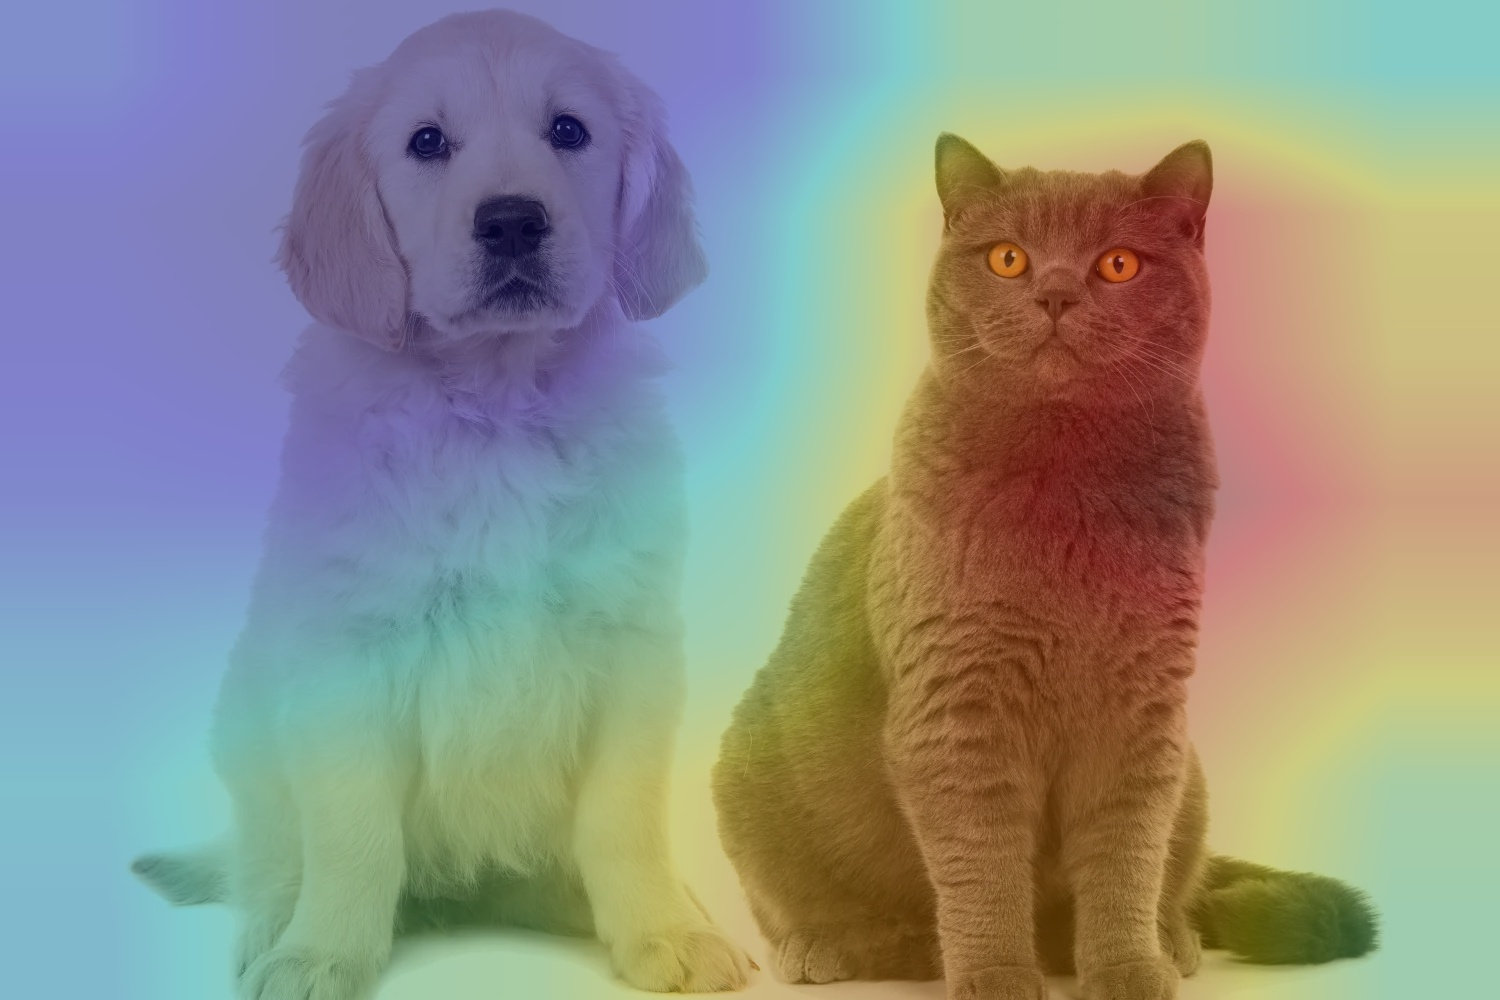
\includegraphics[width=.4\columnwidth]{CAM2.jpg}}
    \qquad
    \subfigure[Ringlet, Score=0.539]{
    \label{fig:Ex3}
    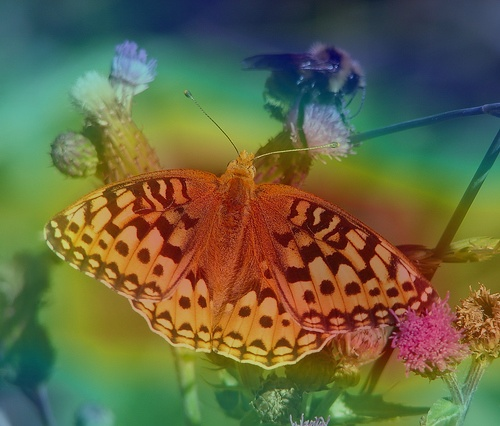
\includegraphics[width=.4\columnwidth]{CAM3.jpg}}
    \qquad
    \subfigure[Bee, Score=0.005]{
    \label{fig:Ex4}
    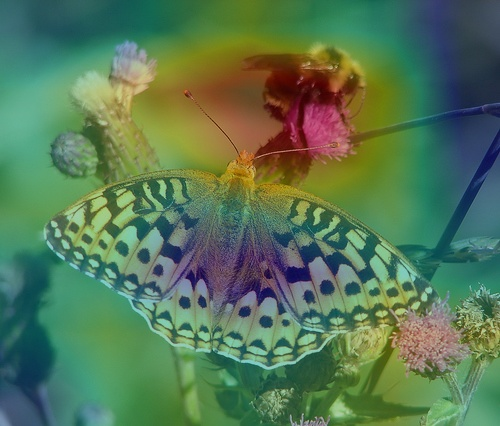
\includegraphics[width=.4\columnwidth]{CAM4.jpg}}
    \caption[Short text]{CAM is class discriminative}
    \label{fig:Defi}
\end{figure}

In case of multiple instances of target object, the performance suffers. It is not able to localise well on each instance.

\begin{figure}[H]
    \centering
    \subfigure[]{
    \label{fig:Ex3}
    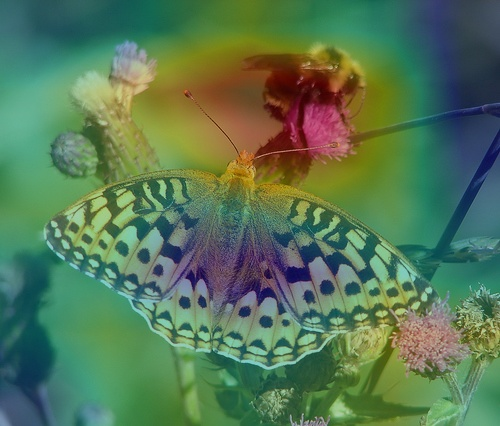
\includegraphics[width=.8\columnwidth]{CAM.jpg}}
    \qquad
    \subfigure[]{
    \label{fig:Ex4}
    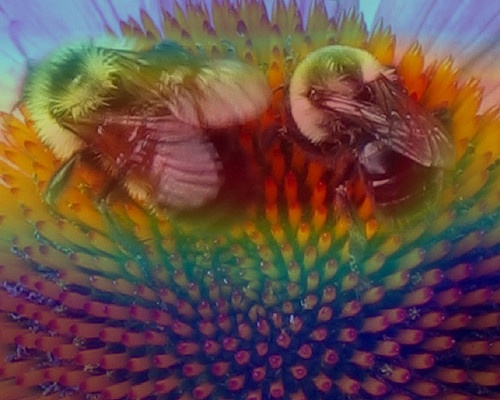
\includegraphics[width=.8\columnwidth]{CAM5 .jpg}}
    \caption[Short text]{The CNN can't localise well in case of multiple objects}
    \label{fig:Defi}
\end{figure}

CAM likely suffered from the use of Global Average Pooling to compute weights. This might be improved by using a conventional pooling layer.   